\section{Βελτιστοποίηση με τη μέθοδο της απότομης καθόδου} % (fold)

Στη μέθοδο της απότομης καθόδου, για την ανανέωση του διανύσματος των μεταβλητών σχεδιασμού, χρησιμοποιείται η σχέση \ref{eq:SD} χρησιμοποιώντας το τοπικό διάνυσμα κλίσης της αντικειμενικής συνάρτησης ως διεύθυνση ανίχνευσης.

\begin{equation}
\begin{aligned}
   \vec{b}^{k+1} =& \vec{b}^{k} + n^k\cdot\vec{p}^k\\
\vec{p}^k = & - \nabla F(x^k)
\end{aligned}
    \label{eq:SD}
\end{equation}

Η τιμή του συντελεστή $n^k$ καθορίζει το βήμα ανίχνευσης στη διεύθυνση $\vec{p}^k$ για το δεδομένη επανάληψη της διαδικασίας. Η τιμή του συντελεστή $n^k$ μπορεί να επιλεγεί δυναμικά, δηλαδή με διαφορετική τιμή για κάθε επανάληψη, δημιουργώντας ενα νεο πρόβλημα βελτιστοποίησης, που αφορά την ελαχιστοποίηση τη νέα τιμή της αντικειμενικής συνάρτησης στο συγκεκριμένο βήμα, μεταβάλλωντας τον συντελεστή $n^k$. Αυτή η προσέγγιση δεν είναι πάντα η καλύτερη, και προφανώς είναι υπολογιστικά πολύ απαιτητική. Μια συχνή προσέγγιση για την επιλογή του $n^k$ σε κάθε βήμα ακολουθεί την εξής λογική. 

\begin{enumerate}
    \item Αρχικοποίηση $n^k$
    \item Διπλασιασμός $n^k$ σε κάθε βήμα
    \item Έλεγχος νέας τιμής της αντικειμενικής συνάρτησης
    \item Αν η νεα τιμή δεν είναι μεγαλύτερη της προηγούμενης -> Βήμα 2
    \item Εναλλακτικά, υποδιπλασιασμός $n^k$
\end{enumerate}

Στο βήμα 4, ο έλεγχος για μείωση της αντικειμενικής συνάρτησης είναι μια απλή προσέγγιση, συχνά χρησιμοποιούνται οι συνθήκες το Wolfe για τον έλεγχο του βήματος. Στην περίπτωσή μας, δοκιμάσαμε μεταβλητό βήμα όπως υποδεικνύεται απο τη μέθοδο που παρουσιάζεται παραπάνω, και συγκρίναμε τη σύγκλιση της λύσης σε σχέση με την περίπτωση σταθερού βήματος. Η τιμή του σταθερού βήματος επιλέχθηκε μετά απο δοκιμές για την τάξη μεγέθους που επιτρέπει μια αρκετά γρήγορη κάθοδο της αντικειμενικής συνάρτησης.

Επομένως, ακολουθώντας την σχέση \ref{eq:SD} υλοποιήσαμε αλγόριθμο που επαναληπτικά υπολογίζει τις νέες τιμές των μεταβλητών σχεδιασμού υπολογίζοντας τις τιμές των παραγώγων ευαισθησίας με καθεμία απο τις μεθόδους που αναλύθηκαν στα προηγούμενα ερωτήματα. Ως κριτήριο τερματισμού του αλγορίθμου, ορίσαμε την διατήρηση σταθερής τιμής αντικειμενικής συνάρτησης για παραπάνω απο 30 επαναλήψεις (idle iterations). Επιπλέον, θέσαμε μέγιστο όριο επαναλήψεων ίσο με 1000. 

Στο σχήμα \ref{fig:adapt} παρατίθεται το διάγραμμα σύγκλισης για σταθερό και μεταβλητό βήμα με παραγώγους υπολογισμένες με πεπερασμένες διαφορές.   

\begin{figure}[h!]
    \begin{center}
        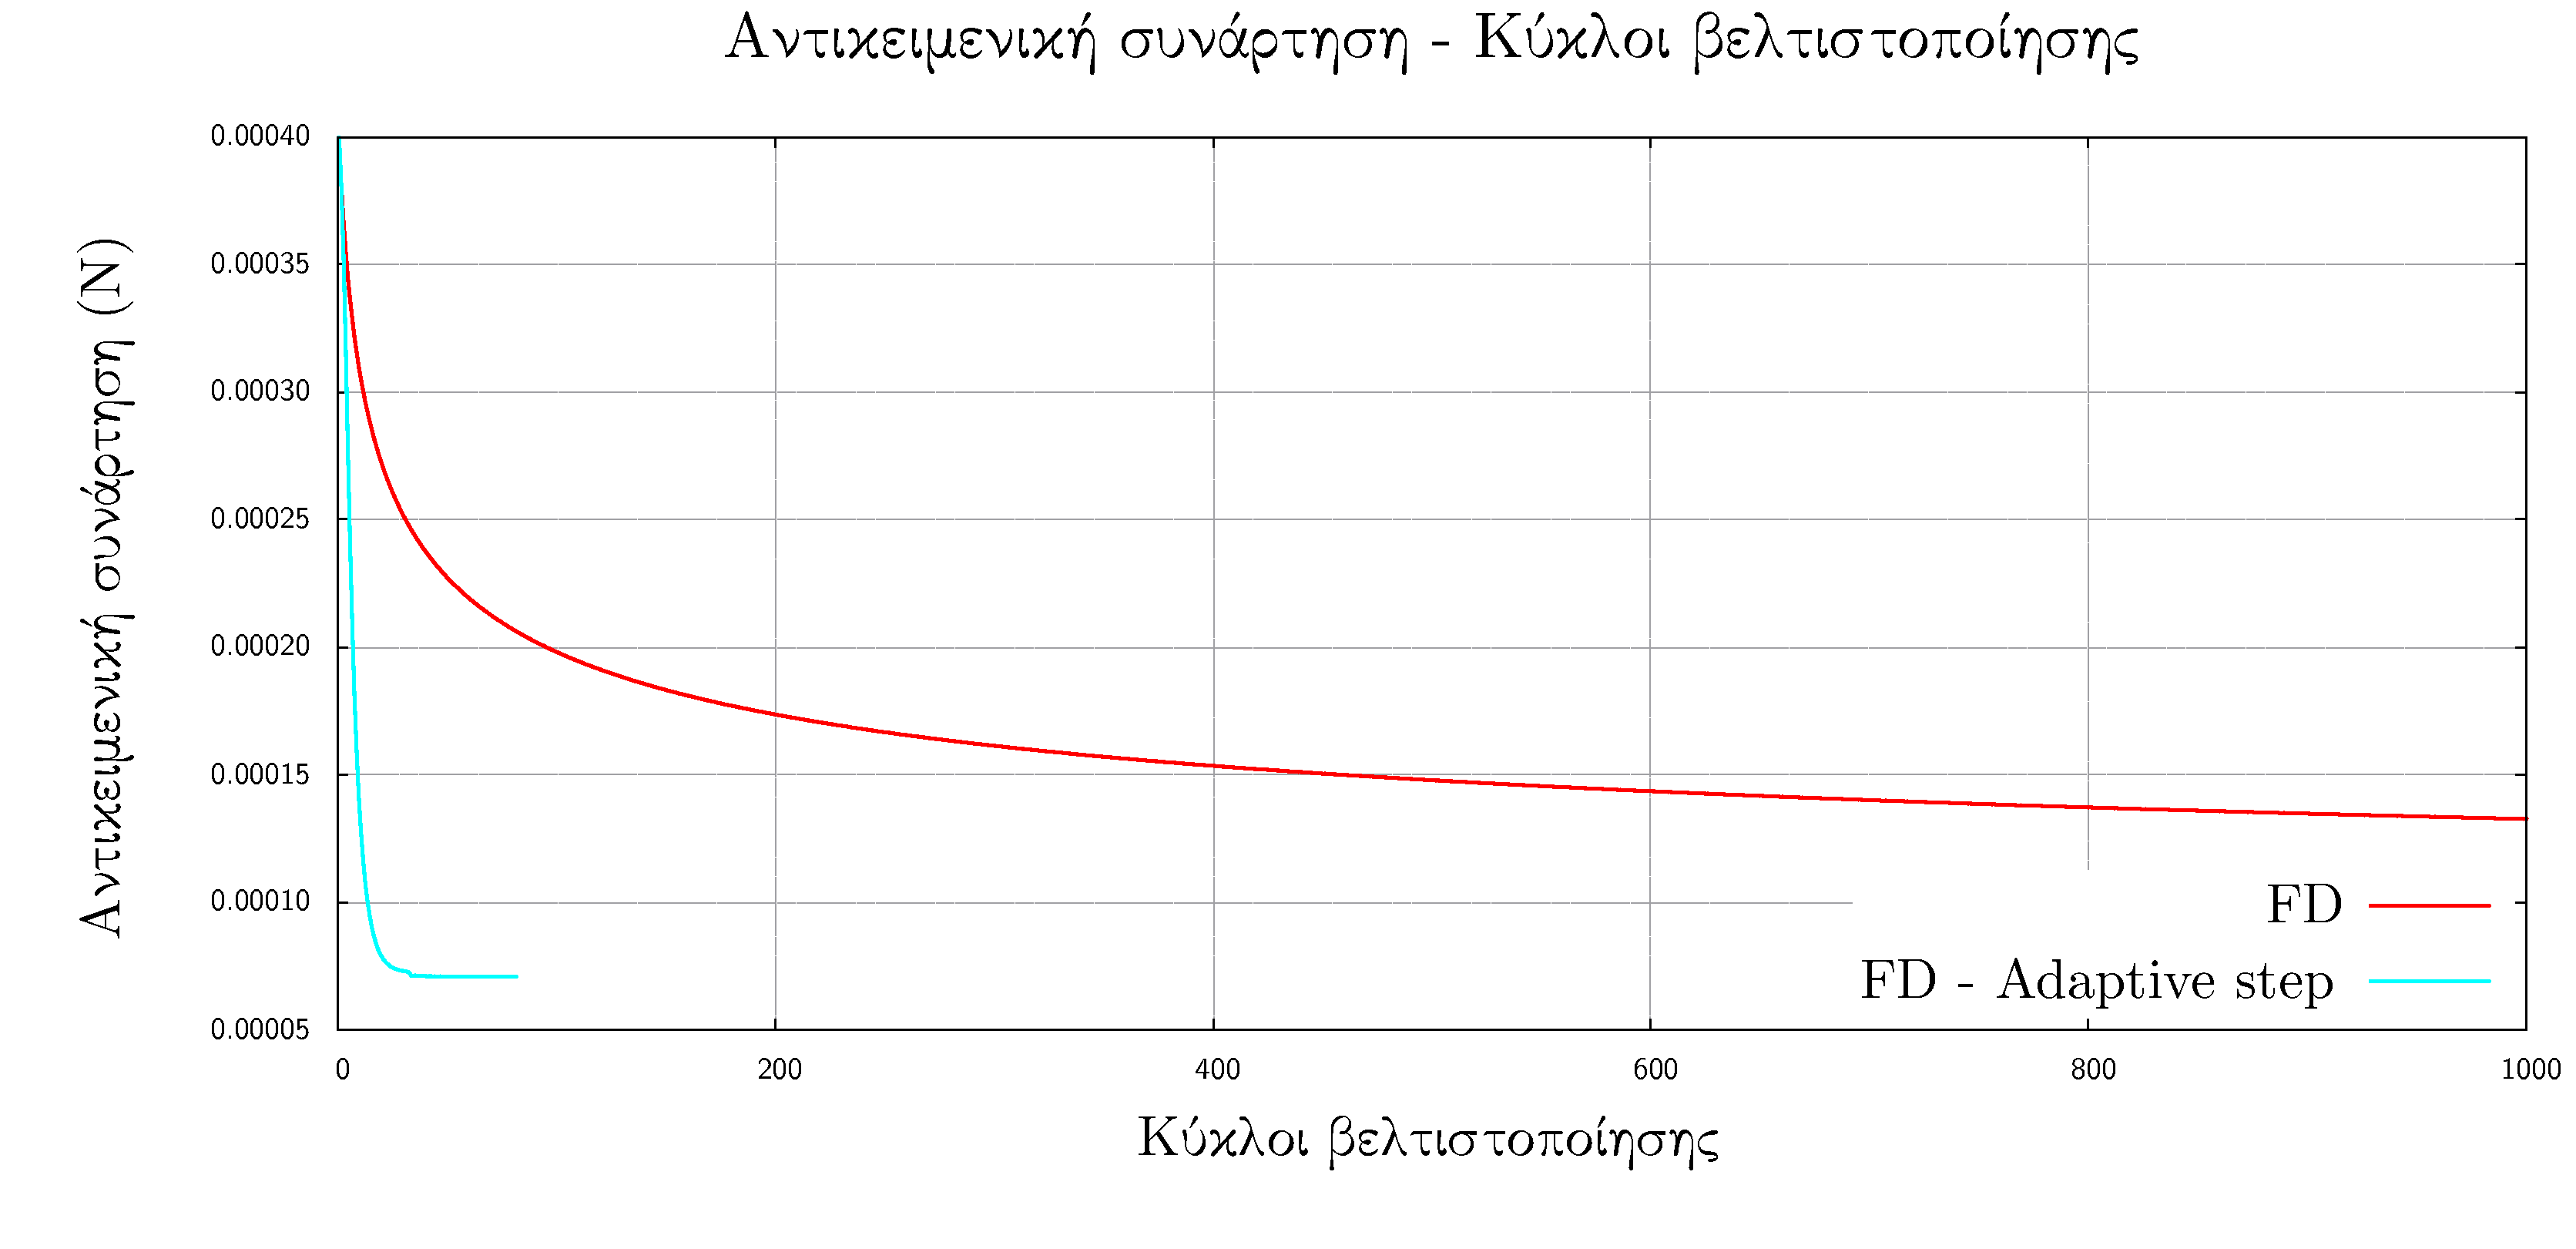
\includegraphics[width=0.95\textwidth]{figures/F_vs_adapt.pdf}
    \end{center}
    \caption{Σύγκριση σταθερού και μεταβλητού βήματος}
    \label{fig:adapt}
\end{figure}

Παρατηρείται πως στην περίπτωση του μεταβλητού βήματος, ο αλγόριθμος μεταβάλλει την τιμή της αντικειμενικής συνάρτησης πολύ πιο γρήγορα, ενώ ο αλγόριθμος σταματάει πολύ πιο νωρίς λόγω του περιορισμού των idle iterations.


Τα τελικά διαγράμματα σύγκλισης για κάθε μέθοδο παρατίθενται στο σχήμα \ref{fig:opt} χρησιμοποιώντας μεταβλητό βήμα. 


\begin{figure}[h!]
    \begin{center}
        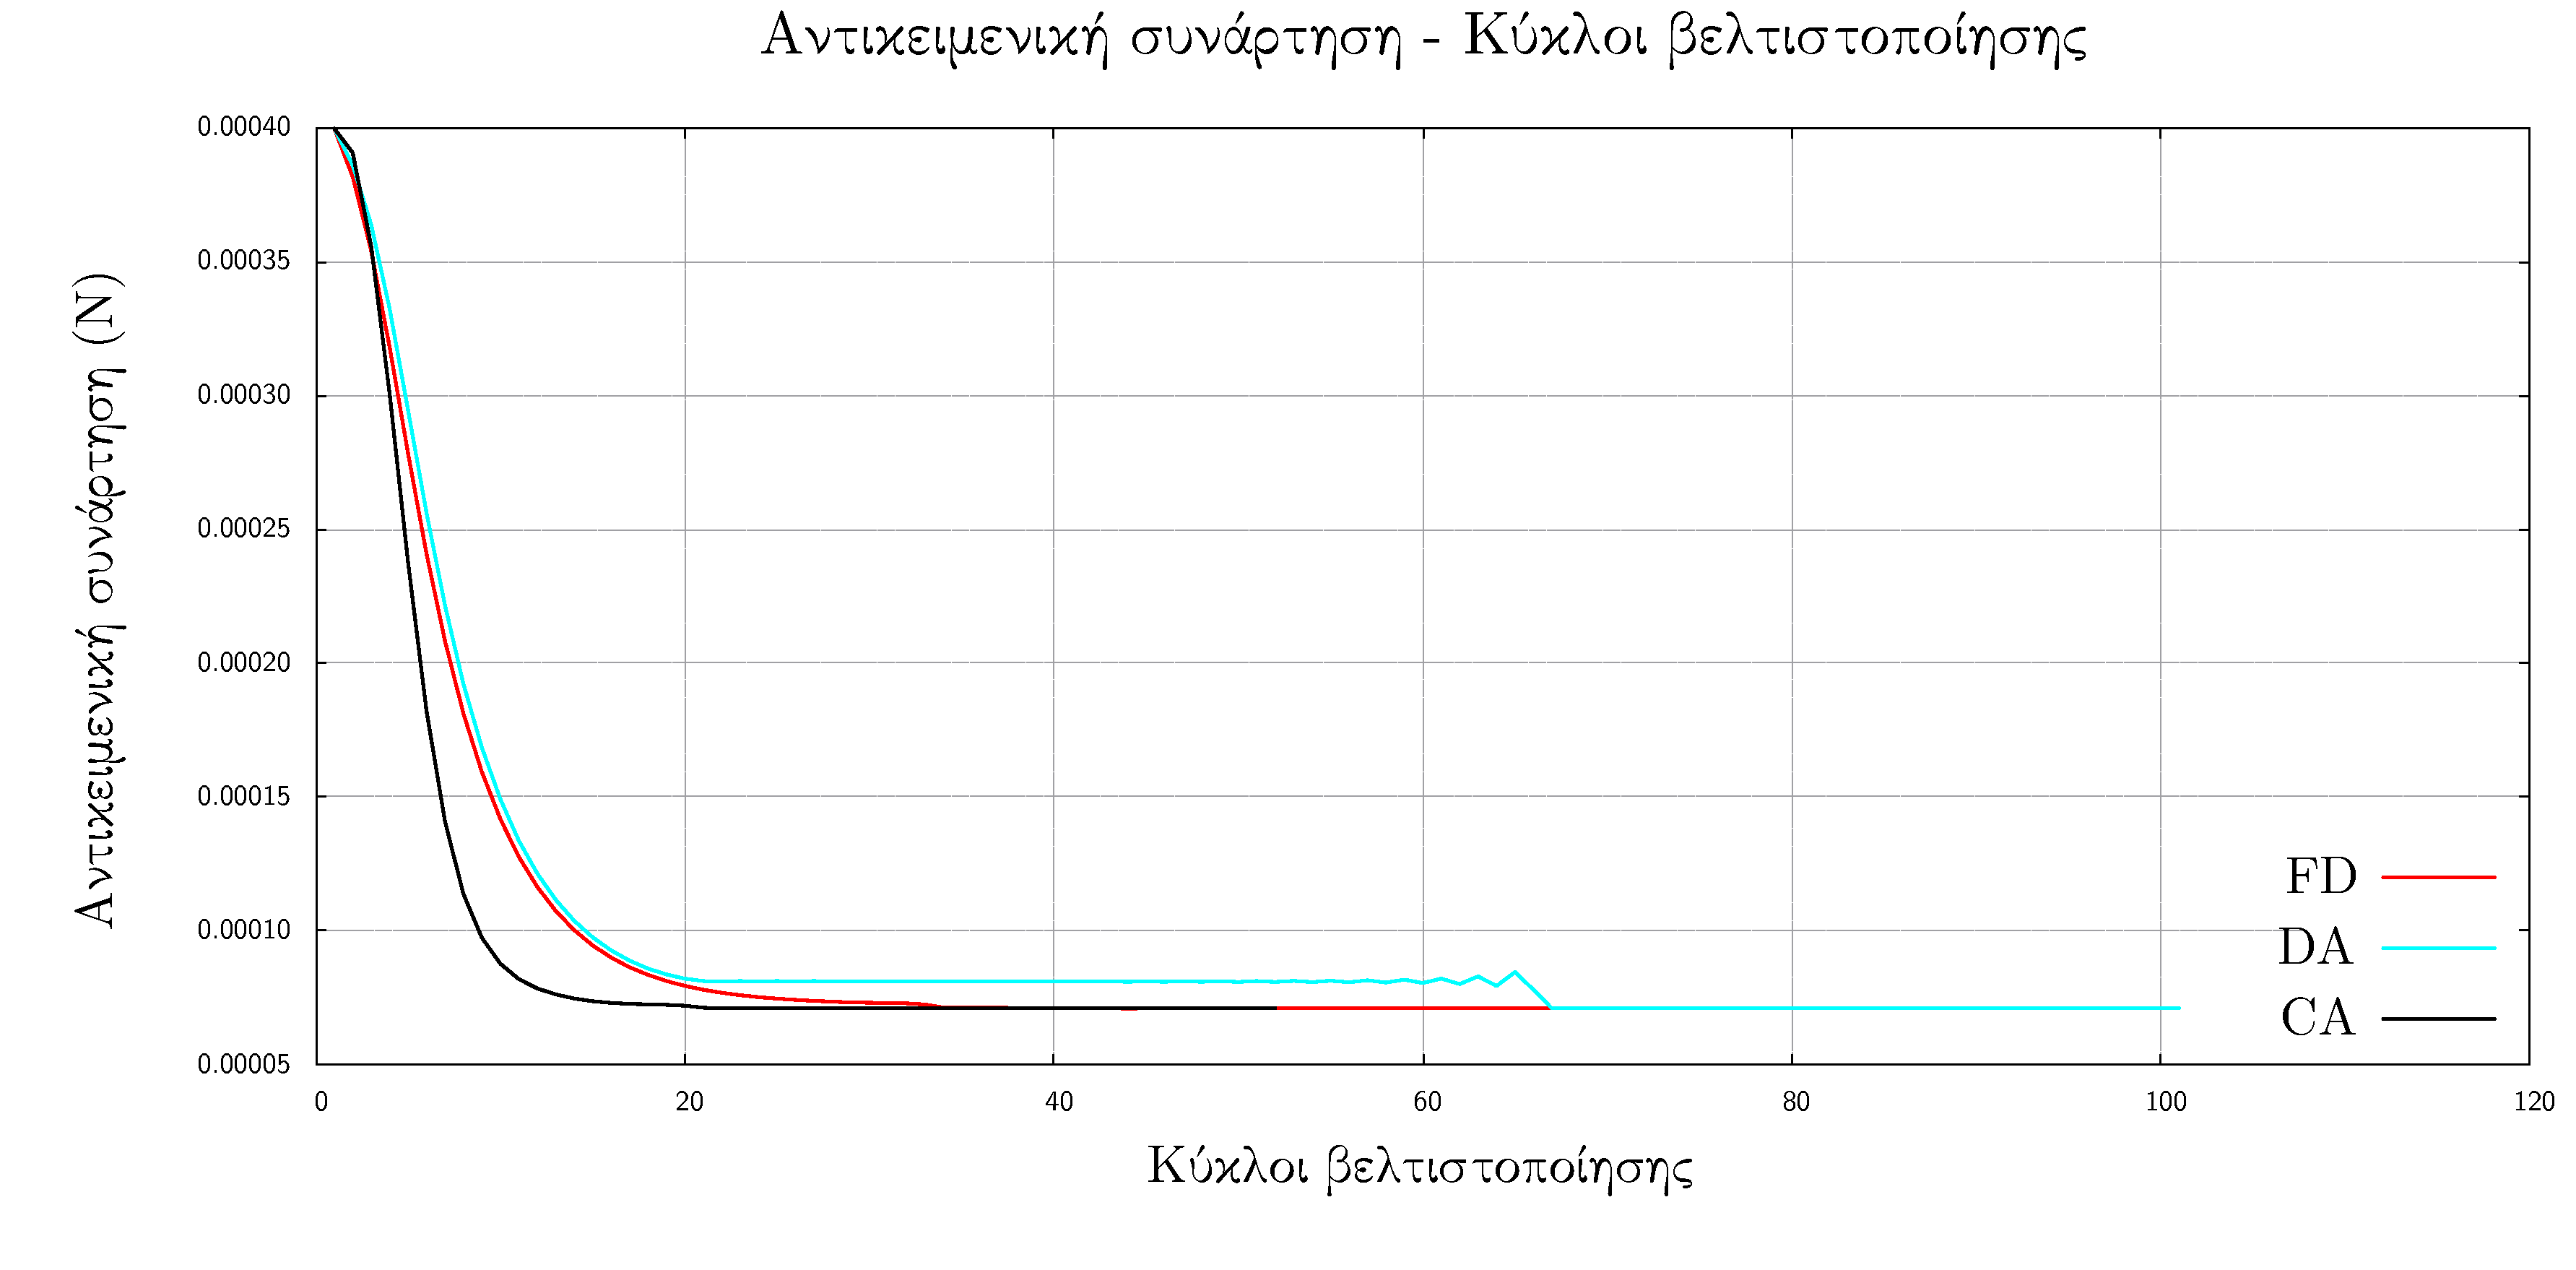
\includegraphics[width=0.95\textwidth]{figures/F_vs_iter.pdf}
    \end{center}
    \caption{Διάγραμμα σύγκλισης για διαφορετικές μεθόδους υπολογισμού παραγώγων}
    \label{fig:opt}
\end{figure}


Όπως αναφέραμε και σε προηγούμενα ερωτήματα, παρατηρούμε πως ξεκινώντας με ίδιες αρχικές μεταβλητές σχεδιασμού, δεν ακολουθούν όλες οι μέθοδοι την ίδια πορεία. Αυτό φυσικά σημαίνει πως υπάρχει διαφορά στις τιμές των παραγώγων που υπολογίζουν οι τρεις μέθοδοι και αποτελεί αίτιο προβληματισμού. Επιπλέον, φαίνεται πως υπάρχει κάποια ταλάντωση στην καμπύλη της διακριτής συζυγής μεθόδου που μπορεί να υποδεικνύει είτε αριθμητική αστάθεια στον υπολογισμό των παραγώγων είτε πολύ μεγάλο βήμα κοντά στο ελάχιστο. Ωστόσο, φαίνεται πως μεχρι το σημείο της αστάθειας, οι καμπύλες της DA, FD βαίνουν πολύ κοντα. Συμφωνώντας με το προηγούμενο ερώτημα, η CA φαίνεται να υπολογίζει αρκετά διαφορετικές παραγώγους αφου παρουσιάζει σημαντικά διαφορετική καμπύλη. 

Σημειώνεται τέλος, πως η συγκεκριμένη αντικειμενική συνάρτηση δεν παρουσιάζει ελάχιστο και μειώνεται όσο αυξάνουμε τις τιμές των μεταβλητών σχεδιασμού. Ο περιορισμός στην παροχή αναγκαζει τις πρώτες τρείς μεταβλητές να αυξάνονται όσο η τέταρτη μειώνεται. Λόγω της σύμβασης του προσήμου για την παροχή, αυτό υποδεικνύει πως η τριβή ελαχιστοποιείται εκχέοντας μεγάλες ταχύτητες στην αρχή της πλάκας και απορροφώντας αντίστοιχα μεγάλες ποσότητες στο τέλος της. 


